\documentclass[xcolor={dvipsnames, svgnames, x11names, table}, 10pt]{beamer}
\usepackage{./assets/preamble}

\title{Programmazione generica e \texttt{STL}}
\date{5 ottobre 2021}
\institute{Università degli Studi di Trento}

% arara: xelatex: { synctex: no }
% arara: xelatex: { synctex: yes }
% arara: latexmk: { clean: partial }
\begin{document}

\frame{\titlepage}

\section*{Riassunto lezione precedente}

\begin{frame}{Argomenti trattati nell'ultima lezione}

    \begin{itemize}
        \item Programmazione generica, template e introduzione STL;
        \item STL: esempi di uso contentitori.
    \end{itemize}

\end{frame}

\section{Contenitori}

\begin{frame}{Contenitori}

    \begin{itemize}
        \item sono Template che \enquote{contengono} altri tipi parametrici;
        \item il contenuto si accede usando gli iterativi.
    \end{itemize}

\end{frame}

\begin{frame}[c]{Iteratori}

    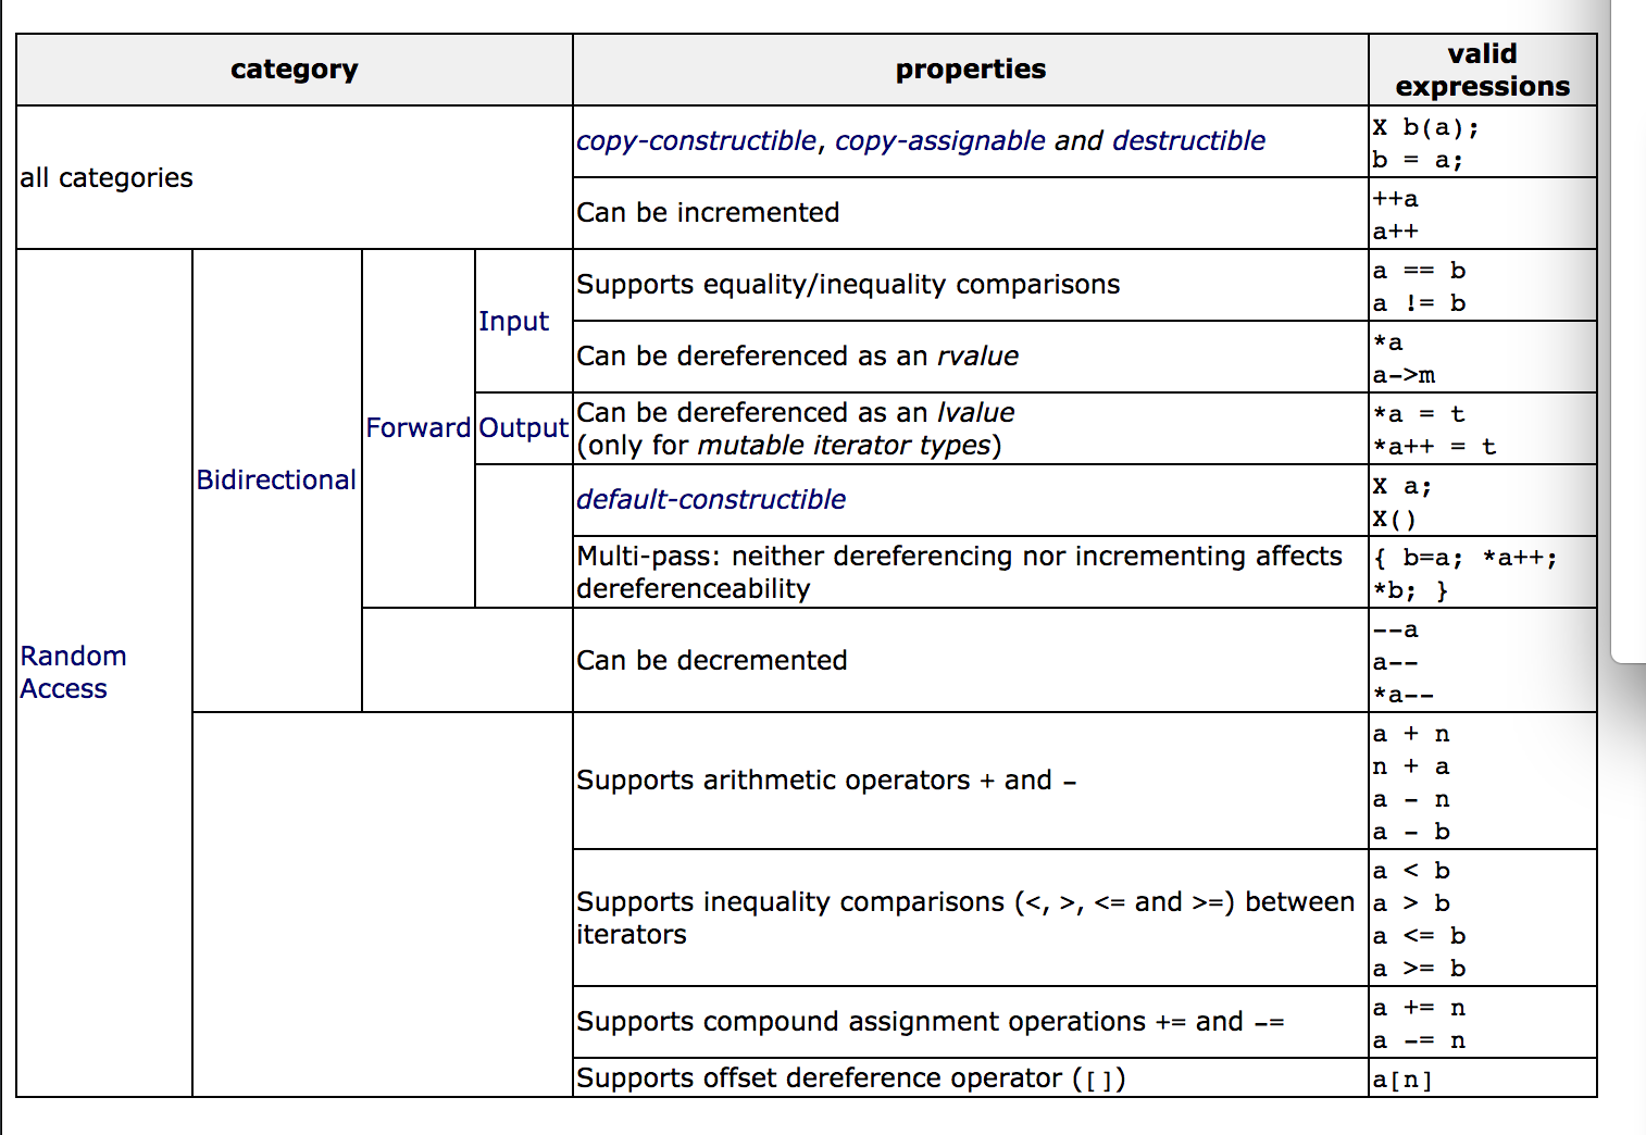
\includegraphics[width=\textwidth, trim={0.2cm 0.55cm 0.75cm 0.5cm}, clip]{iterators}

\end{frame}

\begin{frame}[t, fragile]{list [1/6]}

    \cppfilepath[lastline=9]{Esempio0/main1-original.cpp}

\end{frame}

\begin{frame}[t, fragile]{list [2/7]}

    \cppfilepath[firstline=11, lastline=26]{Esempio0/main1-original.cpp}
    
    \begin{center}
        \texttt{32323243}
    \end{center}

\end{frame}

\begin{frame}[t, fragile]{list [3/6]}

\begin{columns}

\column{0.7\textwidth}
    \cppfilepath[firstline=30, lastline=45]{Esempio0/main1-original.cpp}

\column{0.3\textwidth}
    \texttt{43}
    
    \texttt{5432}
    
    \texttt{43}
    
    \texttt{743}
    
    \texttt{743743}
    
\end{columns}

\end{frame}

\begin{frame}[t, fragile]{list [4/6]}

\begin{columns}
    
\column{0.7\textwidth}
    \cppfilepath[firstline=49, lastline=62]{Esempio0/main1-original.cpp}

\column{0.3\textwidth}
    \texttt{l:98743743}
    
    \texttt{7}
    
    \texttt{l:98}
    \texttt{l2:743743}
    
    \texttt{l:743743}\\
    \texttt{l2:98}
    
\end{columns}

\end{frame}

\begin{frame}[t, fragile]{list [5/6]}

\begin{columns}
    
\column{0.7\textwidth}
    \cppfilepath[firstline=66, lastline=81]{Esempio0/main1-original.cpp}

\column{0.3\textwidth}
    \texttt{6}\texttt{0}
    
    \texttt{l:347347}\\
    \texttt{l:334477}\\
    \texttt{l:347}
    
    \texttt{l:34789}\\
    \texttt{l2:}
    
\end{columns}

\end{frame}

\begin{frame}[t, fragile]{list [5/6]}

\begin{columns}
    
\column{0.7\textwidth}
    \cppfilepath[firstline=85, lastline=107]{Esempio0/main1-original.cpp}

\column{0.3\textwidth}
    \texttt{9874398743}
    
    \texttt{l:3478}
    
    \texttt{l:478}
    
    \texttt{l:78}
    
    \texttt{l:1178}
    
    \texttt{l:131178}
    
    \texttt{l2:1178}
    
\end{columns}

\end{frame}

\begin{frame}[t, fragile]{list [6/6]}

\cppfilepath[firstline=111, lastline=121]{Esempio0/main1-original.cpp}

    \texttt{l3:131178}
    
    \texttt{l:1178}
    
    \texttt{l2:1178}
    
    \texttt{l:768614336404564650}

\end{frame}

\begin{frame}{Operazioni non viste sulle liste}
    
    \begin{itemize}
        \item \textbf{\texttt{emplace\_front}}
        \item \textbf{\texttt{emplace\_back}}
        \item \textbf{\texttt{set\_allocator}}
        \item \textbf{\texttt{crbegin}}
        \item \textbf{\texttt{crend}}
    \end{itemize}
    
\end{frame}

\section{Set e Map}

\begin{frame}[t, fragile]{Set e map}

\begin{itemize}
    \item Sono ordinati e usano \texttt{operator<};
    \item \textbf{non} hanno il concetto di \enquote{front} e \enquote{back};
    \item si usa \texttt{insert}
\end{itemize}

\begin{minted}{cpp}
Class A{ };

set<A> s;

s.insert(A()); // funziona solo se definito A::operator<

map<A,int> m;

m.insert(pair<A,int> (A(),2));
// funziona solo se definito A::operator<

map<int,A> ma;

ma.insert(pair<int,A> (3,A()));
// funziona, operator< definito per gli int tipo base

ma[3] = A(); // equivalentemente per il map è ridefinito operator[]
\end{minted}

\end{frame}

\subsection{Esempio con codice}

\subsubsection{film}

\begin{frame}{\texttt{film.h}}

    \cppfilepath[firstline=9, lastline=23]{Esempio1/film.h}
    
\end{frame}

\begin{frame}{\texttt{film.cpp}}

    \cppfilepath{Esempio1/film.cpp}
    
\end{frame}

\subsubsection{spettatore}

\begin{frame}{\texttt{spettatore.h}}

    \cppfilepath[fontsize=\tiny]{Esempio1/spettatore.h}
    
\end{frame}

\begin{frame}{\texttt{spettatore.cpp} [1/2]}

\begin{columns}
    \column{\dimexpr\paperwidth-30pt}
    \cppfilepath[lastline=24]{Esempio1/spettatore.cpp}
\end{columns}
    
\end{frame}

\begin{frame}{\texttt{spettatore.cpp} [2/2]}
    
    \cppfilepath[firstline=26]{Esempio1/spettatore.cpp}
    
\end{frame}

\subsubsection{cineteca}

\begin{frame}{\texttt{cineteca.h}}
    
    \cppfilepath{Esempio1/cineteca.h}
    
\end{frame}

\begin{frame}[fragile]{\texttt{cineteca.cpp} [1/2]}
    
    \cppfilepath[lastline=21]{Esempio1/cineteca.cpp}
    
    \begin{minted}[linenos=false]{cpp}
    // continua...
    \end{minted}
    
\end{frame}

\begin{frame}{\texttt{cineteca.cpp} [2/2]}
    
    \cppfilepath[firstline=23]{Esempio1/cineteca.cpp}
    
\end{frame}

\subsubsection{main}

\begin{frame}{\texttt{main.cpp}}
    
    \cppfilepath{Esempio1/main.cpp}
    
\end{frame}

\section{Multiset e multimap}

\begin{frame}[fragile]{Multiset e multimap}

Come \texttt{set} e \texttt{map} ma permettendo valori multipli, inotre nel \texttt{multimap} non c'è \texttt{operator[]}.

\end{frame}

\subsection{Esempio con codice}

\subsubsection{fraction}

\begin{frame}[fragile]{\texttt{fraction.h} [1/2]}

    \cppfilepath[lastline=20]{Esempio2/fraction.h}
    
    \begin{minted}[linenos=false]{cpp}
    // continua...
    \end{minted}
    
\end{frame}

\begin{frame}{\texttt{fraction.h} [2/2]}

\begin{columns}
    \column{\dimexpr\paperwidth-30pt}
    \cppfilepath[firstline=21]{Esempio2/fraction.h}
\end{columns}

\end{frame}

\begin{frame}{\texttt{fraction.cpp} [1/11]}
    
    \cppfilepath[lastline=17]{Esempio2/fraction.cpp}
    
\end{frame}

\begin{frame}{\texttt{fraction.cpp} [2/11]}
    
    \cppfilepath[firstline=19, lastline=32]{Esempio2/fraction.cpp}
    
\end{frame}

\begin{frame}{\texttt{fraction.cpp} [3/11]}
    
    \cppfilepath[firstline=34, lastline=48]{Esempio2/fraction.cpp}
    
\end{frame}

\begin{frame}{\texttt{fraction.cpp} [4/11]}
    
    \cppfilepath[firstline=50, lastline=76, fontsize=\tiny]{Esempio2/fraction.cpp}
    
\end{frame}

\begin{frame}{\texttt{fraction.cpp} [5/11]}
    
    \cppfilepath[firstline=78, lastline=109, fontsize=\tiny]{Esempio2/fraction.cpp}
    
\end{frame}

\begin{frame}[fragile]{\texttt{fraction.cpp} [6/11]}
    
    \cppfilepath[firstline=111, lastline=119]{Esempio2/fraction.cpp}
    \begin{minted}[texcomments, linenos=false]{cpp}
    // [logica nella prossima slide]
    \end{minted}
    \cppfilepath[firstline=145, lastline=146]{Esempio2/fraction.cpp}
    
\end{frame}

\begin{frame}{\texttt{fraction.cpp} [7/11]}
    
    \cppfilepath[firstline=120, lastline=144]{Esempio2/fraction.cpp}
    
\end{frame}

\begin{frame}{\texttt{fraction.cpp} [8/11]}
    
    \cppfilepath[firstline=148, lastline=172]{Esempio2/fraction.cpp}
    
\end{frame}

\begin{frame}{\texttt{fraction.cpp} [9/11]}
    
    \cppfilepath[firstline=174, lastline=199]{Esempio2/fraction.cpp}
    
\end{frame}

\begin{frame}{\texttt{fraction.cpp} [10/11]}
    
    \cppfilepath[firstline=201, lastline=223]{Esempio2/fraction.cpp}
    
\end{frame}

\begin{frame}{\texttt{fraction.cpp} [11/11]}
    
    \cppfilepath[firstline=225, lastline=231]{Esempio2/fraction.cpp}
    
\end{frame}

\Riconoscimenti

\end{document}